% Options for packages loaded elsewhere
\PassOptionsToPackage{unicode}{hyperref}
\PassOptionsToPackage{hyphens}{url}
\PassOptionsToPackage{dvipsnames,svgnames,x11names}{xcolor}
%
\documentclass[
  11pt,
  a4paper,
  DIV=11,
  numbers=noendperiod]{scrartcl}

\usepackage{amsmath,amssymb}
\usepackage{iftex}
\ifPDFTeX
  \usepackage[T1]{fontenc}
  \usepackage[utf8]{inputenc}
  \usepackage{textcomp} % provide euro and other symbols
\else % if luatex or xetex
  \usepackage{unicode-math}
  \defaultfontfeatures{Scale=MatchLowercase}
  \defaultfontfeatures[\rmfamily]{Ligatures=TeX,Scale=1}
\fi
\usepackage{lmodern}
\ifPDFTeX\else  
    % xetex/luatex font selection
\fi
% Use upquote if available, for straight quotes in verbatim environments
\IfFileExists{upquote.sty}{\usepackage{upquote}}{}
\IfFileExists{microtype.sty}{% use microtype if available
  \usepackage[]{microtype}
  \UseMicrotypeSet[protrusion]{basicmath} % disable protrusion for tt fonts
}{}
\makeatletter
\@ifundefined{KOMAClassName}{% if non-KOMA class
  \IfFileExists{parskip.sty}{%
    \usepackage{parskip}
  }{% else
    \setlength{\parindent}{0pt}
    \setlength{\parskip}{6pt plus 2pt minus 1pt}}
}{% if KOMA class
  \KOMAoptions{parskip=half}}
\makeatother
\usepackage{xcolor}
\usepackage[lmargin=2cm,rmargin=2cm,tmargin=2cm,bmargin=2cm]{geometry}
\setlength{\emergencystretch}{3em} % prevent overfull lines
\setcounter{secnumdepth}{-\maxdimen} % remove section numbering
% Make \paragraph and \subparagraph free-standing
\ifx\paragraph\undefined\else
  \let\oldparagraph\paragraph
  \renewcommand{\paragraph}[1]{\oldparagraph{#1}\mbox{}}
\fi
\ifx\subparagraph\undefined\else
  \let\oldsubparagraph\subparagraph
  \renewcommand{\subparagraph}[1]{\oldsubparagraph{#1}\mbox{}}
\fi

\usepackage{color}
\usepackage{fancyvrb}
\newcommand{\VerbBar}{|}
\newcommand{\VERB}{\Verb[commandchars=\\\{\}]}
\DefineVerbatimEnvironment{Highlighting}{Verbatim}{commandchars=\\\{\}}
% Add ',fontsize=\small' for more characters per line
\usepackage{framed}
\definecolor{shadecolor}{RGB}{241,243,245}
\newenvironment{Shaded}{\begin{snugshade}}{\end{snugshade}}
\newcommand{\AlertTok}[1]{\textcolor[rgb]{0.68,0.00,0.00}{#1}}
\newcommand{\AnnotationTok}[1]{\textcolor[rgb]{0.37,0.37,0.37}{#1}}
\newcommand{\AttributeTok}[1]{\textcolor[rgb]{0.40,0.45,0.13}{#1}}
\newcommand{\BaseNTok}[1]{\textcolor[rgb]{0.68,0.00,0.00}{#1}}
\newcommand{\BuiltInTok}[1]{\textcolor[rgb]{0.00,0.23,0.31}{#1}}
\newcommand{\CharTok}[1]{\textcolor[rgb]{0.13,0.47,0.30}{#1}}
\newcommand{\CommentTok}[1]{\textcolor[rgb]{0.37,0.37,0.37}{#1}}
\newcommand{\CommentVarTok}[1]{\textcolor[rgb]{0.37,0.37,0.37}{\textit{#1}}}
\newcommand{\ConstantTok}[1]{\textcolor[rgb]{0.56,0.35,0.01}{#1}}
\newcommand{\ControlFlowTok}[1]{\textcolor[rgb]{0.00,0.23,0.31}{#1}}
\newcommand{\DataTypeTok}[1]{\textcolor[rgb]{0.68,0.00,0.00}{#1}}
\newcommand{\DecValTok}[1]{\textcolor[rgb]{0.68,0.00,0.00}{#1}}
\newcommand{\DocumentationTok}[1]{\textcolor[rgb]{0.37,0.37,0.37}{\textit{#1}}}
\newcommand{\ErrorTok}[1]{\textcolor[rgb]{0.68,0.00,0.00}{#1}}
\newcommand{\ExtensionTok}[1]{\textcolor[rgb]{0.00,0.23,0.31}{#1}}
\newcommand{\FloatTok}[1]{\textcolor[rgb]{0.68,0.00,0.00}{#1}}
\newcommand{\FunctionTok}[1]{\textcolor[rgb]{0.28,0.35,0.67}{#1}}
\newcommand{\ImportTok}[1]{\textcolor[rgb]{0.00,0.46,0.62}{#1}}
\newcommand{\InformationTok}[1]{\textcolor[rgb]{0.37,0.37,0.37}{#1}}
\newcommand{\KeywordTok}[1]{\textcolor[rgb]{0.00,0.23,0.31}{#1}}
\newcommand{\NormalTok}[1]{\textcolor[rgb]{0.00,0.23,0.31}{#1}}
\newcommand{\OperatorTok}[1]{\textcolor[rgb]{0.37,0.37,0.37}{#1}}
\newcommand{\OtherTok}[1]{\textcolor[rgb]{0.00,0.23,0.31}{#1}}
\newcommand{\PreprocessorTok}[1]{\textcolor[rgb]{0.68,0.00,0.00}{#1}}
\newcommand{\RegionMarkerTok}[1]{\textcolor[rgb]{0.00,0.23,0.31}{#1}}
\newcommand{\SpecialCharTok}[1]{\textcolor[rgb]{0.37,0.37,0.37}{#1}}
\newcommand{\SpecialStringTok}[1]{\textcolor[rgb]{0.13,0.47,0.30}{#1}}
\newcommand{\StringTok}[1]{\textcolor[rgb]{0.13,0.47,0.30}{#1}}
\newcommand{\VariableTok}[1]{\textcolor[rgb]{0.07,0.07,0.07}{#1}}
\newcommand{\VerbatimStringTok}[1]{\textcolor[rgb]{0.13,0.47,0.30}{#1}}
\newcommand{\WarningTok}[1]{\textcolor[rgb]{0.37,0.37,0.37}{\textit{#1}}}

\providecommand{\tightlist}{%
  \setlength{\itemsep}{0pt}\setlength{\parskip}{0pt}}\usepackage{longtable,booktabs,array}
\usepackage{calc} % for calculating minipage widths
% Correct order of tables after \paragraph or \subparagraph
\usepackage{etoolbox}
\makeatletter
\patchcmd\longtable{\par}{\if@noskipsec\mbox{}\fi\par}{}{}
\makeatother
% Allow footnotes in longtable head/foot
\IfFileExists{footnotehyper.sty}{\usepackage{footnotehyper}}{\usepackage{footnote}}
\makesavenoteenv{longtable}
\usepackage{graphicx}
\makeatletter
\def\maxwidth{\ifdim\Gin@nat@width>\linewidth\linewidth\else\Gin@nat@width\fi}
\def\maxheight{\ifdim\Gin@nat@height>\textheight\textheight\else\Gin@nat@height\fi}
\makeatother
% Scale images if necessary, so that they will not overflow the page
% margins by default, and it is still possible to overwrite the defaults
% using explicit options in \includegraphics[width, height, ...]{}
\setkeys{Gin}{width=\maxwidth,height=\maxheight,keepaspectratio}
% Set default figure placement to htbp
\makeatletter
\def\fps@figure{htbp}
\makeatother

\KOMAoption{captions}{tableheading}
\makeatletter
\makeatother
\makeatletter
\makeatother
\makeatletter
\@ifpackageloaded{caption}{}{\usepackage{caption}}
\AtBeginDocument{%
\ifdefined\contentsname
  \renewcommand*\contentsname{Table of contents}
\else
  \newcommand\contentsname{Table of contents}
\fi
\ifdefined\listfigurename
  \renewcommand*\listfigurename{List of Figures}
\else
  \newcommand\listfigurename{List of Figures}
\fi
\ifdefined\listtablename
  \renewcommand*\listtablename{List of Tables}
\else
  \newcommand\listtablename{List of Tables}
\fi
\ifdefined\figurename
  \renewcommand*\figurename{Figure}
\else
  \newcommand\figurename{Figure}
\fi
\ifdefined\tablename
  \renewcommand*\tablename{Table}
\else
  \newcommand\tablename{Table}
\fi
}
\@ifpackageloaded{float}{}{\usepackage{float}}
\floatstyle{ruled}
\@ifundefined{c@chapter}{\newfloat{codelisting}{h}{lop}}{\newfloat{codelisting}{h}{lop}[chapter]}
\floatname{codelisting}{Listing}
\newcommand*\listoflistings{\listof{codelisting}{List of Listings}}
\makeatother
\makeatletter
\@ifpackageloaded{caption}{}{\usepackage{caption}}
\@ifpackageloaded{subcaption}{}{\usepackage{subcaption}}
\makeatother
\makeatletter
\@ifpackageloaded{tcolorbox}{}{\usepackage[skins,breakable]{tcolorbox}}
\makeatother
\makeatletter
\@ifundefined{shadecolor}{\definecolor{shadecolor}{rgb}{.97, .97, .97}}
\makeatother
\makeatletter
\makeatother
\makeatletter
\makeatother
\ifLuaTeX
  \usepackage{selnolig}  % disable illegal ligatures
\fi
\IfFileExists{bookmark.sty}{\usepackage{bookmark}}{\usepackage{hyperref}}
\IfFileExists{xurl.sty}{\usepackage{xurl}}{} % add URL line breaks if available
\urlstyle{same} % disable monospaced font for URLs
\hypersetup{
  pdftitle={Analysis},
  colorlinks=true,
  linkcolor={blue},
  filecolor={Maroon},
  citecolor={Blue},
  urlcolor={Blue},
  pdfcreator={LaTeX via pandoc}}

\title{Analysis}
\author{}
\date{}

\begin{document}
\maketitle
\ifdefined\Shaded\renewenvironment{Shaded}{\begin{tcolorbox}[interior hidden, borderline west={3pt}{0pt}{shadecolor}, breakable, enhanced, frame hidden, boxrule=0pt, sharp corners]}{\end{tcolorbox}}\fi

\textbf{ARE THE CONVICTS WELL EDUCATED?}

\begin{itemize}
\item
  ARE THE CONVICTS WELL EDUCATED?
\item
  IS THERE INCREASE TREND IN SPECIFIC PRIODS FOR SPECIFIC GROUPS?
\item
  WHY DO WE SEE FLUCTUATION IN SOME GROUP?
\end{itemize}

In our society and through world there is a belief which claims convicts
have low educational level. According to this belief, thanks to
education, some values can be gained by children during school years. Is
it really so? In this work we want to show some analysis and illuminate
if there is a correlation between education level and probability of
committing a crime with the data of TÜİK which include education level
of convicts of Turkish prisons between 1990-2020. Our data include
education level as variable (Illiterate, Literate but not Graduated from
a school, Primary School, Primary Education, Junior High School and
Vocational School at High School Level, Higher Education, Unknown) and
years 1990-2020 as observations. Lines in each plot which are parallel
to x axis point out average value of table's observations.

\begin{Shaded}
\begin{Highlighting}[]
\FunctionTok{library}\NormalTok{(tidyverse)}
\end{Highlighting}
\end{Shaded}

\begin{verbatim}
Warning: package 'tidyverse' was built under R version 4.3.2
\end{verbatim}

\begin{verbatim}
Warning: package 'ggplot2' was built under R version 4.3.2
\end{verbatim}

\begin{verbatim}
Warning: package 'tidyr' was built under R version 4.3.2
\end{verbatim}

\begin{verbatim}
Warning: package 'readr' was built under R version 4.3.2
\end{verbatim}

\begin{verbatim}
Warning: package 'purrr' was built under R version 4.3.2
\end{verbatim}

\begin{verbatim}
Warning: package 'dplyr' was built under R version 4.3.2
\end{verbatim}

\begin{verbatim}
Warning: package 'stringr' was built under R version 4.3.2
\end{verbatim}

\begin{verbatim}
Warning: package 'forcats' was built under R version 4.3.2
\end{verbatim}

\begin{verbatim}
Warning: package 'lubridate' was built under R version 4.3.2
\end{verbatim}

\begin{verbatim}
-- Attaching core tidyverse packages ------------------------ tidyverse 2.0.0 --
v dplyr     1.1.4     v readr     2.1.4
v forcats   1.0.0     v stringr   1.5.1
v ggplot2   3.4.4     v tibble    3.2.1
v lubridate 1.9.3     v tidyr     1.3.0
v purrr     1.0.2     
-- Conflicts ------------------------------------------ tidyverse_conflicts() --
x dplyr::filter() masks stats::filter()
x dplyr::lag()    masks stats::lag()
i Use the conflicted package (<http://conflicted.r-lib.org/>) to force all conflicts to become errors
\end{verbatim}

\begin{Shaded}
\begin{Highlighting}[]
\FunctionTok{load}\NormalTok{(}\StringTok{"\textasciitilde{}/Github/emu430{-}fall2023{-}team{-}data\_criminals/data\_criminals.RData"}\NormalTok{)}
\NormalTok{average\_illiterate}\OtherTok{=}\FunctionTok{mean}\NormalTok{(data\_criminals}\SpecialCharTok{$}\NormalTok{Illiterate)}
\FunctionTok{ggplot}\NormalTok{(data\_criminals,}\FunctionTok{aes}\NormalTok{(...}\DecValTok{1}\NormalTok{,Illiterate))}\SpecialCharTok{+}\FunctionTok{geom\_point}\NormalTok{(}\AttributeTok{color=}\StringTok{"green"}\NormalTok{)}\SpecialCharTok{+}\FunctionTok{theme}\NormalTok{(}\AttributeTok{axis.text.x =} \FunctionTok{element\_text}\NormalTok{(}\AttributeTok{angle =} \DecValTok{90}\NormalTok{, }\AttributeTok{hjust =} \DecValTok{1}\NormalTok{))}\SpecialCharTok{+}\FunctionTok{labs}\NormalTok{(}\AttributeTok{title =} \StringTok{"Illiterate over Years"}\NormalTok{, }\AttributeTok{x =} \StringTok{"Years"}\NormalTok{, }\AttributeTok{y =} \StringTok{"Number of Illiterates"}\NormalTok{)}\SpecialCharTok{+}\FunctionTok{geom\_hline}\NormalTok{(}\AttributeTok{yintercept =}\NormalTok{ average\_illiterate, }\AttributeTok{col =} \StringTok{"green"}\NormalTok{)}
\end{Highlighting}
\end{Shaded}

\begin{figure}[H]

{\centering 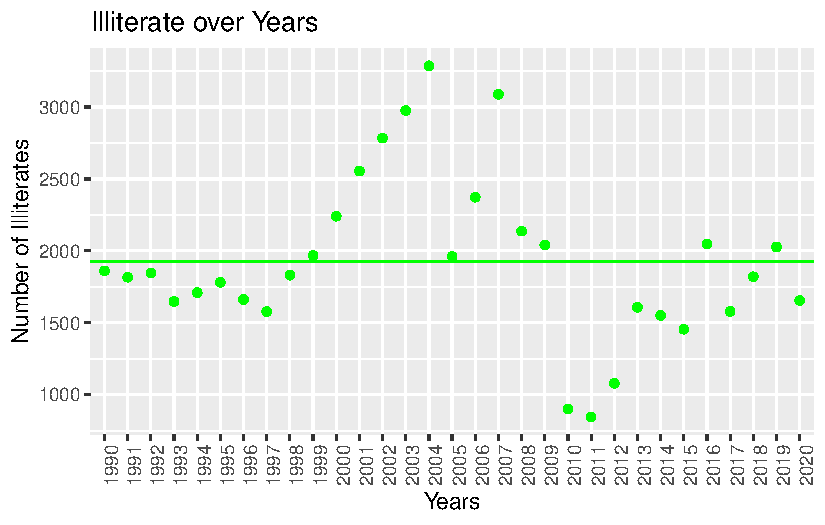
\includegraphics{analysis_files/figure-pdf/unnamed-chunk-1-1.pdf}

}

\end{figure}

As seen on the plot between 1997-2004 years there is a increase trend
and in 2010, 2011, 2012 are lowest numbers for illiterate. We can see
fluctuation over the years and interestingly compared to other education
levels, number of illiterates has lowest average. Rates of illiterates
of Turkey is important to make a interpretation and it is subject of
another research. Our data provide only education level of convicts.

\begin{Shaded}
\begin{Highlighting}[]
\NormalTok{average\_literates}\OtherTok{=}\FunctionTok{mean}\NormalTok{(data\_criminals}\SpecialCharTok{$}\StringTok{\textasciigrave{}}\AttributeTok{Literate but not Graduated from a School}\StringTok{\textasciigrave{}}\NormalTok{)}
\FunctionTok{ggplot}\NormalTok{(data\_criminals,}\FunctionTok{aes}\NormalTok{(...}\DecValTok{1}\NormalTok{,data\_criminals}\SpecialCharTok{$}\StringTok{\textasciigrave{}}\AttributeTok{Literate but not Graduated from a School}\StringTok{\textasciigrave{}}\NormalTok{ ))}\SpecialCharTok{+}\FunctionTok{geom\_point}\NormalTok{(}\AttributeTok{color=}\StringTok{"red"}\NormalTok{)}\SpecialCharTok{+}\FunctionTok{theme}\NormalTok{(}\AttributeTok{axis.text.x =} \FunctionTok{element\_text}\NormalTok{(}\AttributeTok{angle =} \DecValTok{90}\NormalTok{, }\AttributeTok{hjust =} \DecValTok{1}\NormalTok{))}\SpecialCharTok{+}\FunctionTok{labs}\NormalTok{(}\AttributeTok{title =} \StringTok{"Literate over Years"}\NormalTok{, }\AttributeTok{x =} \StringTok{"Years"}\NormalTok{, }\AttributeTok{y =} \StringTok{"Number of Literates"}\NormalTok{)}\SpecialCharTok{+}\FunctionTok{geom\_hline}\NormalTok{(}\AttributeTok{yintercept =}\NormalTok{ average\_literates, }\AttributeTok{col =} \StringTok{"red"}\NormalTok{)}
\end{Highlighting}
\end{Shaded}

\begin{verbatim}
Warning: Use of `` data_criminals$`Literate but not Graduated from a School` `` is
discouraged.
i Use `Literate but not Graduated from a School` instead.
\end{verbatim}

\begin{figure}[H]

{\centering 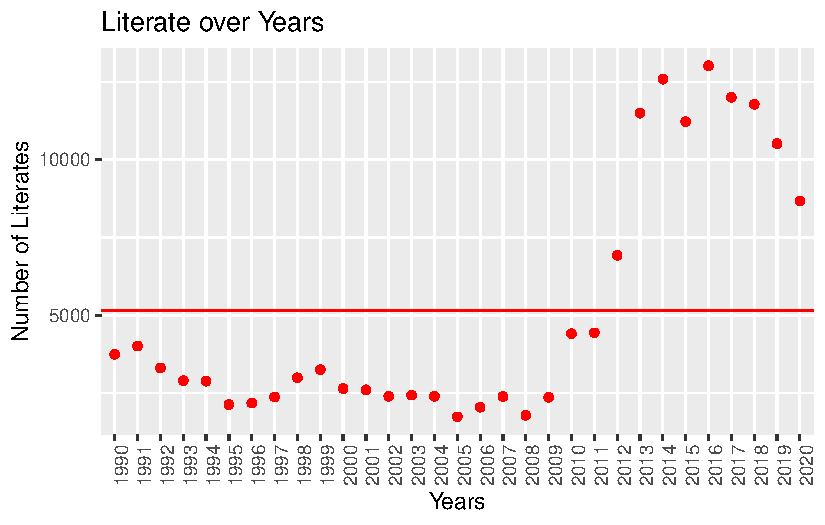
\includegraphics{analysis_files/figure-pdf/unnamed-chunk-2-1.pdf}

}

\end{figure}

When we look at the number of literates who have not graduated from a
school, we can see increase after 2009 and their average find its
position at third.

\begin{Shaded}
\begin{Highlighting}[]
\NormalTok{data\_criminals}\SpecialCharTok{$}\StringTok{\textasciigrave{}}\AttributeTok{Primary Education}\StringTok{\textasciigrave{}}\NormalTok{[}\FunctionTok{is.na}\NormalTok{(data\_criminals}\SpecialCharTok{$}\StringTok{\textasciigrave{}}\AttributeTok{Primary Education}\StringTok{\textasciigrave{}}\NormalTok{)] }\OtherTok{\textless{}{-}} \DecValTok{0}
\NormalTok{p}\OtherTok{=}\NormalTok{data\_criminals}\SpecialCharTok{\%\textgreater{}\%} \FunctionTok{mutate}\NormalTok{(}\AttributeTok{Primary=}\StringTok{\textasciigrave{}}\AttributeTok{Primary School}\StringTok{\textasciigrave{}}\SpecialCharTok{+}\StringTok{\textasciigrave{}}\AttributeTok{Primary Education}\StringTok{\textasciigrave{}}\NormalTok{)}
\NormalTok{average\_primary}\OtherTok{=}\FunctionTok{mean}\NormalTok{(p}\SpecialCharTok{$}\NormalTok{Primary)}
\FunctionTok{ggplot}\NormalTok{(p,}\FunctionTok{aes}\NormalTok{(...}\DecValTok{1}\NormalTok{,Primary))}\SpecialCharTok{+}\FunctionTok{geom\_point}\NormalTok{(}\AttributeTok{color=}\StringTok{"brown"}\NormalTok{)}\SpecialCharTok{+}\FunctionTok{theme}\NormalTok{(}\AttributeTok{axis.text.x =} \FunctionTok{element\_text}\NormalTok{(}\AttributeTok{angle =} \DecValTok{90}\NormalTok{, }\AttributeTok{hjust =} \DecValTok{1}\NormalTok{))}\SpecialCharTok{+}\FunctionTok{labs}\NormalTok{(}\AttributeTok{title =} \StringTok{"Number of Graduated from Primary School or Education over Years"}\NormalTok{, }\AttributeTok{x =} \StringTok{"Years"}\NormalTok{, }\AttributeTok{y =} \StringTok{"Number of Primary Education or Primary Scool"}\NormalTok{)}\SpecialCharTok{+}\FunctionTok{geom\_hline}\NormalTok{(}\AttributeTok{yintercept =}\NormalTok{ average\_primary, }\AttributeTok{col =} \StringTok{"brown"}\NormalTok{)}
\end{Highlighting}
\end{Shaded}

\begin{figure}[H]

{\centering 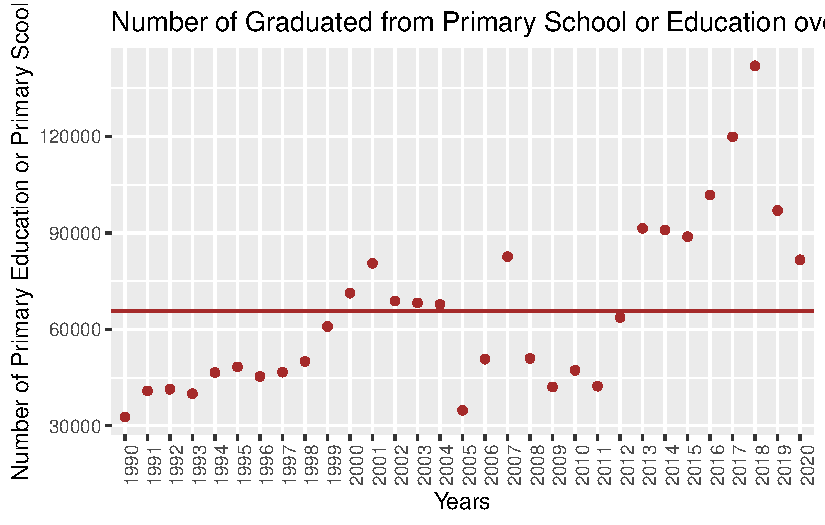
\includegraphics{analysis_files/figure-pdf/unnamed-chunk-3-1.pdf}

}

\end{figure}

In our data frame Primary Education and Primary School has 2 different
column. We combined two column into one column as Primary. We can see
fluctuation over years and increase after 2016. Most probably, sharp
decline after 2018 results from regulation in execution law because of
COVID-19 pandemic. This group has the highest average.

\begin{Shaded}
\begin{Highlighting}[]
\NormalTok{average\_junior\_high\_school}\OtherTok{=}\FunctionTok{mean}\NormalTok{(data\_criminals}\SpecialCharTok{$}\StringTok{\textasciigrave{}}\AttributeTok{Junior High School and Vocational School at Junior High School Level}\StringTok{\textasciigrave{}}\NormalTok{)}
\FunctionTok{ggplot}\NormalTok{(data\_criminals,}\FunctionTok{aes}\NormalTok{(...}\DecValTok{1}\NormalTok{,data\_criminals}\SpecialCharTok{$}\StringTok{\textasciigrave{}}\AttributeTok{Junior High School and Vocational School at Junior High School Level}\StringTok{\textasciigrave{}}\NormalTok{))}\SpecialCharTok{+}\FunctionTok{geom\_point}\NormalTok{(}\AttributeTok{color=}\StringTok{"black"}\NormalTok{)}\SpecialCharTok{+}\FunctionTok{theme}\NormalTok{(}\AttributeTok{axis.text.x =} \FunctionTok{element\_text}\NormalTok{(}\AttributeTok{angle =} \DecValTok{90}\NormalTok{, }\AttributeTok{hjust =} \DecValTok{1}\NormalTok{))}\SpecialCharTok{+}\FunctionTok{labs}\NormalTok{(}\AttributeTok{title =} \StringTok{"Junior High School over Years"}\NormalTok{, }\AttributeTok{x =} \StringTok{"Years"}\NormalTok{, }\AttributeTok{y =} \StringTok{"Number of Junior High School"}\NormalTok{)}\SpecialCharTok{+}\FunctionTok{geom\_hline}\NormalTok{(}\AttributeTok{yintercept =}\NormalTok{ average\_junior\_high\_school, }\AttributeTok{col =} \StringTok{"black"}\NormalTok{)}
\end{Highlighting}
\end{Shaded}

\begin{verbatim}
Warning: Use of `` data_criminals$`Junior High School and Vocational School at Junior
High School Level` `` is discouraged.
i Use `Junior High School and Vocational School at Junior High School Level`
  instead.
\end{verbatim}

\begin{figure}[H]

{\centering 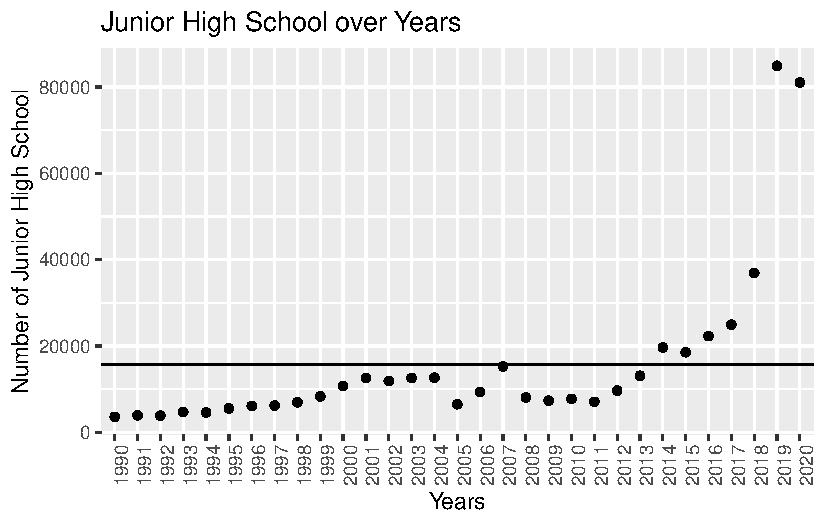
\includegraphics{analysis_files/figure-pdf/unnamed-chunk-4-1.pdf}

}

\end{figure}

As seen on the table there is an increase trend after 2016. Their
average is at the highest forth.

\begin{Shaded}
\begin{Highlighting}[]
\NormalTok{average\_high\_school}\OtherTok{=}\FunctionTok{mean}\NormalTok{(data\_criminals}\SpecialCharTok{$}\StringTok{\textasciigrave{}}\AttributeTok{High School and Vocational School at High School Level}\StringTok{\textasciigrave{}}\NormalTok{)}
\FunctionTok{ggplot}\NormalTok{(data\_criminals,}\FunctionTok{aes}\NormalTok{(...}\DecValTok{1}\NormalTok{,data\_criminals}\SpecialCharTok{$}\StringTok{\textasciigrave{}}\AttributeTok{High School and Vocational School at High School Level}\StringTok{\textasciigrave{}}\NormalTok{))}\SpecialCharTok{+}\FunctionTok{geom\_point}\NormalTok{(}\AttributeTok{color=}\StringTok{"purple"}\NormalTok{)}\SpecialCharTok{+}\FunctionTok{theme}\NormalTok{(}\AttributeTok{axis.text.x =} \FunctionTok{element\_text}\NormalTok{(}\AttributeTok{angle =} \DecValTok{90}\NormalTok{, }\AttributeTok{hjust =} \DecValTok{1}\NormalTok{))}\SpecialCharTok{+}\FunctionTok{labs}\NormalTok{(}\AttributeTok{title =} \StringTok{"High School over Years"}\NormalTok{, }\AttributeTok{x =} \StringTok{"Years"}\NormalTok{, }\AttributeTok{y =} \StringTok{"Number of Convict Graduated from High School"}\NormalTok{)}\SpecialCharTok{+}\FunctionTok{geom\_hline}\NormalTok{(}\AttributeTok{yintercept =}\NormalTok{ average\_junior\_high\_school, }\AttributeTok{col =} \StringTok{"purple"}\NormalTok{)}
\end{Highlighting}
\end{Shaded}

\begin{verbatim}
Warning: Use of `` data_criminals$`High School and Vocational School at High School
Level` `` is discouraged.
i Use `High School and Vocational School at High School Level` instead.
\end{verbatim}

\begin{figure}[H]

{\centering 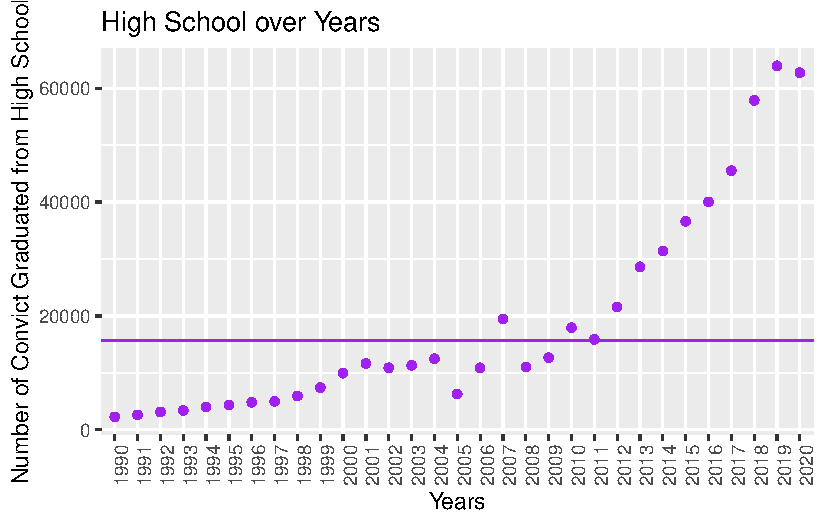
\includegraphics{analysis_files/figure-pdf/unnamed-chunk-5-1.pdf}

}

\end{figure}

Like junior high school numbers, convicts graduated from high school has
an increase trend after 2011. Their average is at the highest 5.

\begin{Shaded}
\begin{Highlighting}[]
\NormalTok{average\_higher\_edu}\OtherTok{=}\FunctionTok{mean}\NormalTok{(data\_criminals}\SpecialCharTok{$}\StringTok{\textasciigrave{}}\AttributeTok{Higher Education}\StringTok{\textasciigrave{}}\NormalTok{)}
\FunctionTok{ggplot}\NormalTok{(data\_criminals,}\FunctionTok{aes}\NormalTok{(...}\DecValTok{1}\NormalTok{,data\_criminals}\SpecialCharTok{$}\StringTok{\textasciigrave{}}\AttributeTok{Higher Education}\StringTok{\textasciigrave{}}\NormalTok{))}\SpecialCharTok{+}\FunctionTok{geom\_point}\NormalTok{(}\AttributeTok{color=}\StringTok{"blue"}\NormalTok{)}\SpecialCharTok{+}\FunctionTok{theme}\NormalTok{(}\AttributeTok{axis.text.x =} \FunctionTok{element\_text}\NormalTok{(}\AttributeTok{angle =} \DecValTok{90}\NormalTok{, }\AttributeTok{hjust =} \DecValTok{1}\NormalTok{))}\SpecialCharTok{+}\FunctionTok{labs}\NormalTok{(}\AttributeTok{title =} \StringTok{"Higher Education over Years"}\NormalTok{, }\AttributeTok{x =} \StringTok{"Years"}\NormalTok{, }\AttributeTok{y =} \StringTok{"Number of Convicts with Higher Education"}\NormalTok{)}\SpecialCharTok{+}\FunctionTok{geom\_hline}\NormalTok{(}\AttributeTok{yintercept =}\NormalTok{average\_higher\_edu , }\AttributeTok{col =} \StringTok{"blue"}\NormalTok{)}
\end{Highlighting}
\end{Shaded}

\begin{verbatim}
Warning: Use of `` data_criminals$`Higher Education` `` is discouraged.
i Use `Higher Education` instead.
\end{verbatim}

\begin{figure}[H]

{\centering 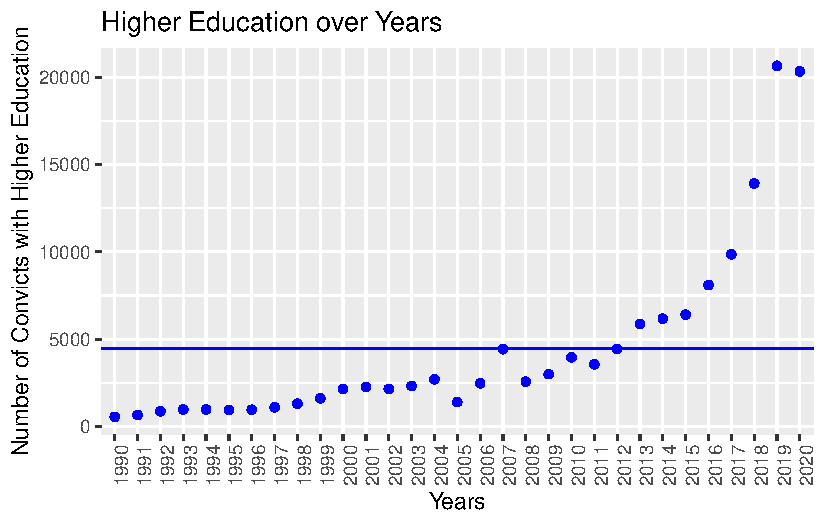
\includegraphics{analysis_files/figure-pdf/unnamed-chunk-6-1.pdf}

}

\end{figure}

Like High School there is a over-increase in the number of convicts who
has higher education after 2016.

As we see in last three plot, there is a increase for Higher Education,
High School and Junior High School after 2016. After failed coup attempt
in 2016, many people were arrested because of political issues and it
can be seen in plots. Fluctuation in some group can be seen in some
plot. These fluctuations results from regulation in execution law,
regulation in criminal law or probation.

Plot shown above does not reflect result of our main objective. We want
to illuminate correlation between education level and crime in Turkey
prisons. Below you can see total number of each education level and
their Pie chart presentation.

\begin{Shaded}
\begin{Highlighting}[]
\NormalTok{total\_ill}\OtherTok{=}\FunctionTok{sum}\NormalTok{(data\_criminals}\SpecialCharTok{$}\NormalTok{Illiterate)}
\NormalTok{total\_lit}\OtherTok{=}\FunctionTok{sum}\NormalTok{(data\_criminals}\SpecialCharTok{$}\StringTok{\textasciigrave{}}\AttributeTok{Literate but not Graduated from a School}\StringTok{\textasciigrave{}}\NormalTok{)}
\NormalTok{total\_pri}\OtherTok{=}\FunctionTok{sum}\NormalTok{(p}\SpecialCharTok{$}\NormalTok{Primary)}
\NormalTok{total\_jhs}\OtherTok{=}\FunctionTok{sum}\NormalTok{(data\_criminals}\SpecialCharTok{$}\StringTok{\textasciigrave{}}\AttributeTok{Junior High School and Vocational School at Junior High School Level}\StringTok{\textasciigrave{}}\NormalTok{)}
\NormalTok{total\_hig}\OtherTok{=}\FunctionTok{sum}\NormalTok{(data\_criminals}\SpecialCharTok{$}\StringTok{\textasciigrave{}}\AttributeTok{High School and Vocational School at High School Level}\StringTok{\textasciigrave{}}\NormalTok{)}
\NormalTok{total\_uni}\OtherTok{=}\FunctionTok{sum}\NormalTok{(data\_criminals}\SpecialCharTok{$}\StringTok{\textasciigrave{}}\AttributeTok{Higher Education}\StringTok{\textasciigrave{}}\NormalTok{)}
\NormalTok{vec}\OtherTok{=}\FunctionTok{c}\NormalTok{(total\_ill,total\_lit,total\_pri,total\_jhs,total\_hig,total\_uni)}
\NormalTok{names\_vec}\OtherTok{=}\FunctionTok{c}\NormalTok{(}\StringTok{"Illiterate"}\NormalTok{,}\StringTok{"Literate"}\NormalTok{,}\StringTok{"Primary"}\NormalTok{,}\StringTok{"J High"}\NormalTok{,}\StringTok{"High Sch"}\NormalTok{,}\StringTok{"High Edu"}\NormalTok{)}
\FunctionTok{names}\NormalTok{(vec)}\OtherTok{=}\NormalTok{names\_vec}
\FunctionTok{barplot}\NormalTok{(vec,}\AttributeTok{main =} \StringTok{"Number of Convicts to Education Level "}\NormalTok{, }\AttributeTok{xlab =} \StringTok{"Education Level"}\NormalTok{, }\AttributeTok{ylab =} \StringTok{"Number of Convicts"}\NormalTok{, }\AttributeTok{border =} \StringTok{"red"}\NormalTok{)}
\end{Highlighting}
\end{Shaded}

\begin{figure}[H]

{\centering 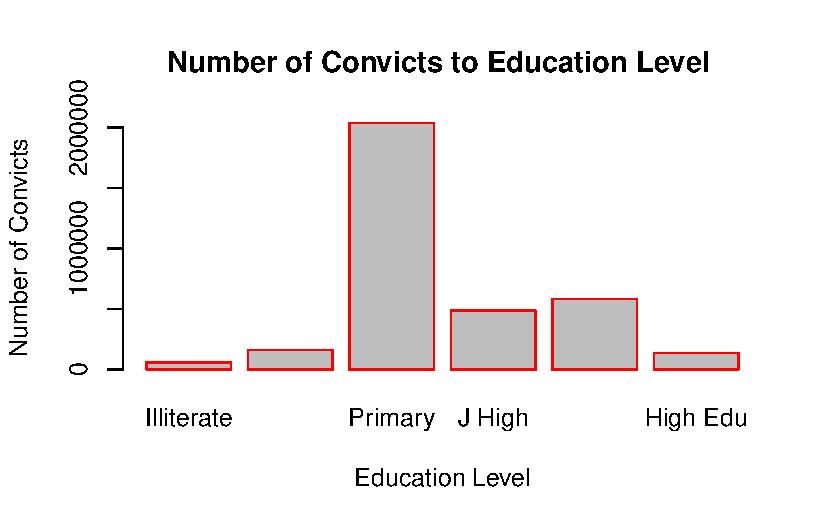
\includegraphics{analysis_files/figure-pdf/unnamed-chunk-7-1.pdf}

}

\end{figure}

\begin{Shaded}
\begin{Highlighting}[]
\NormalTok{rates\_of}\OtherTok{=}\FunctionTok{c}\NormalTok{(}\StringTok{"1.7"}\NormalTok{,}\StringTok{"4.6"}\NormalTok{,}\StringTok{"58.8"}\NormalTok{,}\StringTok{"14.1"}\NormalTok{,}\StringTok{"16.8"}\NormalTok{,}\StringTok{"4"}\NormalTok{)}
\FunctionTok{pie}\NormalTok{(vec, }\AttributeTok{labels =}\NormalTok{ rates\_of, }\AttributeTok{main=}\StringTok{"Pie Chart of Convicts"}\NormalTok{ ,}\AttributeTok{col =} \FunctionTok{rainbow}\NormalTok{(}\FunctionTok{length}\NormalTok{(vec)))}
\FunctionTok{legend}\NormalTok{(}\StringTok{"topright"}\NormalTok{, names\_vec, }\AttributeTok{cex =} \FloatTok{0.8}\NormalTok{,}
   \AttributeTok{fill =} \FunctionTok{rainbow}\NormalTok{(}\FunctionTok{length}\NormalTok{(vec)))}
\end{Highlighting}
\end{Shaded}

\begin{figure}[H]

{\centering 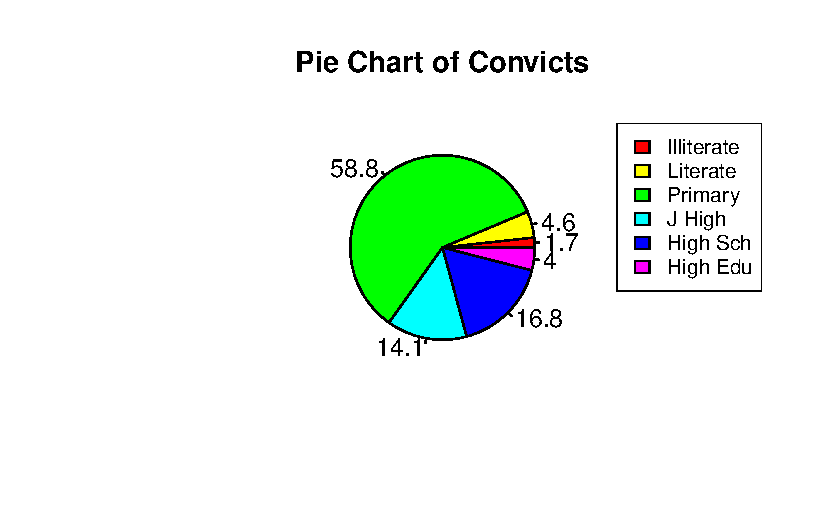
\includegraphics{analysis_files/figure-pdf/unnamed-chunk-8-1.pdf}

}

\end{figure}

As shown on both presentation, convicts education levels and their
numbers between 1990-2020 according to TÜİK's data, More than half of
convicts has primary education. Illiterate and literate convicts make up
only \%6,3 of total number. Convicts, who have higher education, has
only \%4 and junior high school, high school have \%14.1 \%16.8
respectively. In order to be able to say that education level and
probability to commit a crime inversely proportional we need more
evidence. Proportions of education levels in society for each year can
be useful for deep analytics. For example; what the rate of illiterate
people of society for 1995 is can be helpful. Of course these are TÜİK's
data which calculated 2023's inflation rate as \%61,98. As Stalin said
``The death of one person is a tragedy, the death of millions is a
statistic'' and everyone is a little bit manipulative.



\end{document}
